\section{Background \& Motivation}
\label{background}

In this section, we first introduce the background on JavaScript points-to analysis with an example. We then discuss an empirical study of interesting static analysis behavior that guided our design. Finally, we intuitively discuss our approach with the code example.

\subsection{Background}

%The effectiveness of static analysis is often evaluated by its precision and performance. A useful static analysis tool needs to achieve good balance between precision (e.g., low false positive rate) and performance (e.g., completing the analysis under the limited time/space budget). Unfortunately, static program analysis is challenged by specific language features present in the programs (e.g., reflections in Java), overly-approximating the program behavior. A dynamic programming language such as JavaScript is often associated with several of these features. For example, JavaScript allows program constructs to generate code at runtime and supports object property accesses as associative arrays. %Therefore, despite of the efforts on improving the state-of-the-art (e.g., \cite{Sridharan:2012:CTP:2367163.2367191,Andreasen:2014:DSA:2660193.2660214,DBLP:conf/ecoop/ParkR15}), static analysis often experiences scalability and precision problems when analyzing real-world websites that use JavaScript libraries.

Points-to analysis approximates the program's heap by calculating the set of abstract values a variable or reference property may have during execution. Context sensitivity is a general technique to achieve more precise program analysis by distinguishing between calls to a function \cite{sharir1981two}. It has been demonstrated that applying specialized context sensitivity in JavaScript points-to analysis is an effective approach for improving its precision and performance. For example, Sridharan et al. \cite{Sridharan:2012:CTP:2367163.2367191} applies the values of a parameter {\tt p} of a function as the calling context, if {\tt p} is used as the property name in a property access (e.g., {\tt v[p]}), as a special treatment for dynamic property accesses in JavaScript. Because this algorithm is designed to address the challenges caused by a specific language feature, despite the fact that it performs well for the programs where this feature is present, other program constructs from the real-world JavaScript applications may render the analysis ineffective, which require more accurate handling from the static analysis.

%it is intuitive for this algorithm to perform well for the programs where these features are present, while other program constructs may render the analysis ineffective. 

%However, despite of the efforts on improving the state-of-the-art (e.g., \cite{Sridharan:2012:CTP:2367163.2367191,DBLP:conf/ecoop/WeiR14,Andreasen:2014:DSA:2660193.2660214,DBLP:conf/ecoop/ParkR15}), static analysis still experiences scalability and precision problems when analyzing real-world websites that use JavaScript libraries. 

\begin{figure}[th!]
        \lstinputlisting[xleftmargin=20pt]{jquery-modified.js}
\caption{\textmd{Modifed {\tt extend} function of jQuery 1.6.1.}}
\label{fig:jquery-modified}
\end{figure}

Therefore, an important stage of static analysis design is to identify the causes of a static analysis producing unexpected results. We define a {\it root cause} as a program construct that is a source of the precision and/or performance loss for a static analysis. Specifically, if the overall precision and performance of an analysis {\tt A} improves significantly via a specialized handling of the program construct in a specific program location, this construct is the root cause of imprecision of the analysis {\tt A} for the program. For example, Figure \ref{fig:jquery-modified} shows a small piece of code from {\it jQuery}, the most widely used JavaScript library \cite{LibraryUsage}. A whole-program 1-CFA analysis \cite{Shivers:1991:CAH:124950} that separately analyzes each different call site of a function has scalability problems for any simple application that uses {\it jQuery} \cite{Sridharan:2012:CTP:2367163.2367191}. Applying the technique proposed by Sridharan et al. \cite{Sridharan:2012:CTP:2367163.2367191} only for the property accesses at line 5 resolves its performance issues. Therefore, this program construct is a root cause of imprecision of the 1-CFA analysis for {\it jQuery} applications.

Unfortunately, identifying the root causes is a high cost process, requiring extensive experience of static analysis design as well as deep understanding of the target programs. To the best of our knowledge, there is little tool support for this process, making it time-consuming and hard to be comprehensive. For example, identifying the property accesses at line 5 in Figure \ref{fig:jquery-modified} as the root cause for 1-CFA analysis is difficult because (i) the {\it jQuery} library consists of about 9,000 lines of code, and (ii) similar program constructs are used in {\it jQuery}, whereas this particular program location is critical to the overall analysis results. Therefore, we are motivated to develop new techniques to assist in {\it root cause localization} by automating part of the process of identifying the sources of imprecision.

%\footnote{The notion of analysis bottleneck localization is similar to that of {\it fault localization} in software debugging, both being complex and time-consuming processes. While automatic fault localization techniques have been extensively studied \cite{Jones:2005:EET:1101908.1101949}, few work has focused on locating analysis bottlenecks.}

%Static analysis approximates the program behavior via abstractions. For example, points-to analysis, an enabling analysis for various automated software tools, approximates the program's heap by calculating the set of abstract values a variable may have during execution. Performance and precision are two important metrics to evaluate the effectiveness of static analysis algorithms. It is desired for static analysis to achieve good balance between precision (e.g., low false positive rate) and performance (e.g., completing the analysis under a time/space budget). Unfortunately, static program analysis is challenged by specific language features present in the programs (e.g., reflections in Java), overly-approximating the program behavior. A dynamic programming language such as JavaScript is often associated with several of these features. For example, JavaScript allows program constructs to generate code at runtime and supports object property accesses as associative arrays. Therefore, it has been a great challenge to design effective static analysis for JavaScript applications where these dynamic features are present. Static points-to analysis often experiences scalability and precision problems when analyzing websites that use JavaScript libraries.

%Nevertheless, researchers have proposed new approaches that aim to improve the performance and precision of JavaScript static analysis (e.g., \cite{Sridharan:2012:CTP:2367163.2367191,Andreasen:2014:DSA:2660193.2660214,DBLP:conf/ecoop/ParkR15}). These approaches often apply specialized context-sensitive analysis, a general technique to achieve more precise program analysis by distinguishing between calls to a function \cite{sharir1981two}, to reason about the specific dynamic program constructs more accurately. For example, Sridharan et al. \cite{Sridharan:2012:CTP:2367163.2367191} applies the values of a parameter {\tt p} of a function as the calling context, if {\tt p} is used as the property name in a property access (e.g., {\tt v[p]}), as a special treatment of static analysis to accurately handle dynamic property accesses. Despite of the progress on improving the precision and performance of the state-of-the-art JavaScript static analysis, there still exists no static points-to analysis that can accurately analyze real-world websites. A new static analysis approach often produces desirable results for a set of JavaScript applications, while it fails when analyzing other programs. The causes of the undesired static analysis behavior remains to be unveiled.

%Therefore, it is a critical stage of analysis design to investigate and understand why a static analysis cannot produce results with good performance and precision. We define an {\it analysis bottleneck} as a program construct that is a root cause of the loss of precision and/or performance for a static analysis. Specifically, if a more accurate model of the specific program construct in the specific program location results in significant improvement of overall analysis precision and performance, this program construct is the bottleneck for the specific analysis. For example, Figure \ref{fig:jquery-modified} shows a small piece of code from {\it jQuery}, the most widely used JavaScript library. The statement at line 5 is the bottleneck for a 1-CFA analysis when analyzing jQuery applications. If a more precise modeling of only this program construct is used, the 1-CFA analysis becomes scalable. Unfortunately, identifying the analysis bottlenecks relies on expertise of static analysis as well as program understanding, without additional information/help, this process is time consuming and hard to be exhaustive. For example, it is difficult to locate that line 5 is the bottleneck for 1-CFA analysis because (i) jQuery is a program with about 9,000 lines of code and (ii) similar program constructs were used other places in jQuery, but this is the only one that matters; therefore, it is hard to distinguish just based on the features being used. The notion of analysis bottleneck is similar to the notion root cause of faults in software testing. We claim that there is high cost (manual, expertise) for locating analysis bottlenecks in programs, motivated the development of techniques that assist in bottleneck localization by automating part of the process of identifying the analysis bottlenecks.


\subsection{Static Analysis Behavior}

We have performed a brief empirical study to understand the behavior of JavaScript static analysis. Figures \ref{fig:pts-growth} and \ref{fig:pts-distribution} show the different behaviors of two points-to analyses of a simple application that uses {\it jQuery}. The two points-to analyses in comparison are the 0-1-CFA analysis (i.e., only uses 1-CFA analysis for the constructors to name objects by their allocation sites) and the combined 1-CFA and argument-sensitive analysis \cite{Sridharan:2012:CTP:2367163.2367191}. Overall, the 0-1-CFA analysis experiences performance and precision issues (e.g., the analysis cannot finish analyzing the program under 10 minutes), while the combined context-sensitive analysis performs significantly better.

\begin{figure}[th!]
        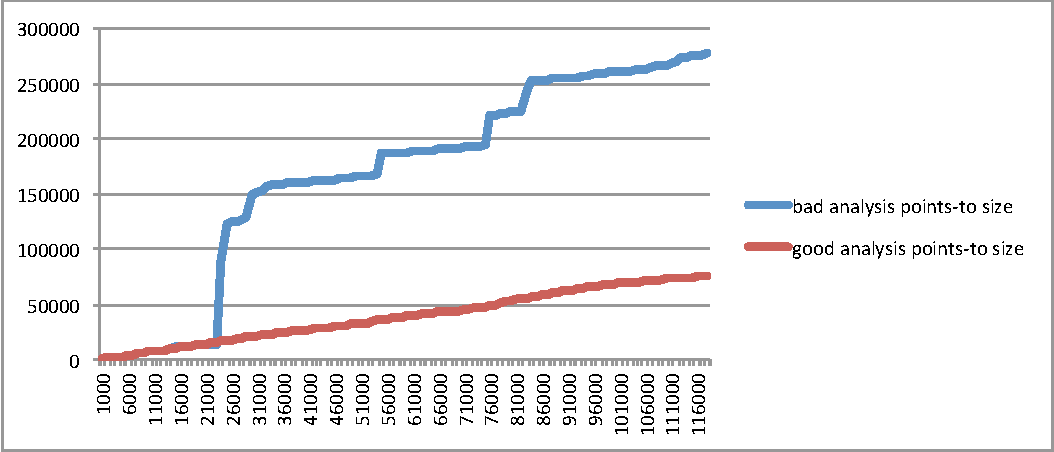
\includegraphics[width=\columnwidth]{pts-growth}
\caption{\textmd{Points-to size growth during the analysis lifetime.}}
\label{fig:pts-growth}
\end{figure}

Figure \ref{fig:pts-growth} shows the trend of overall points-to size (i.e., total number of points-to edges) growth for these two analyses during their lifetimes. The x axis presents the number of evaluations\footnote{An evaluation in the points-to analysis solves a constraint that may result in changes of the points-to results.} and y axis presents the total points-to size of all variables in the program. The good combined context-sensitive analysis' points-to size grows steadily ``linear'' throughout its lifetime. On the other hand, the overall points-to size growth of 0-1-CFA analysis exhibits ``jumps" which are the periods during which its overall points-to size dramatically increases. For example, between evaluations of 23,000 and 25,000, the overall points-to size of the 0-1-CFA analysis grows about ten times. The existence of such ``jumps" indicates that the overly-approximated results are frequently propagated, resulting in significantly overall precision loss. In addition, since the 0-1-CFA analysis experiences scalability issues, it remains incomplete at the end of the allocated analysis time and its overall points-to size keeps growing after the 120,000 evaluations in Figure \ref{fig:pts-growth}.

\begin{figure}[th!]
        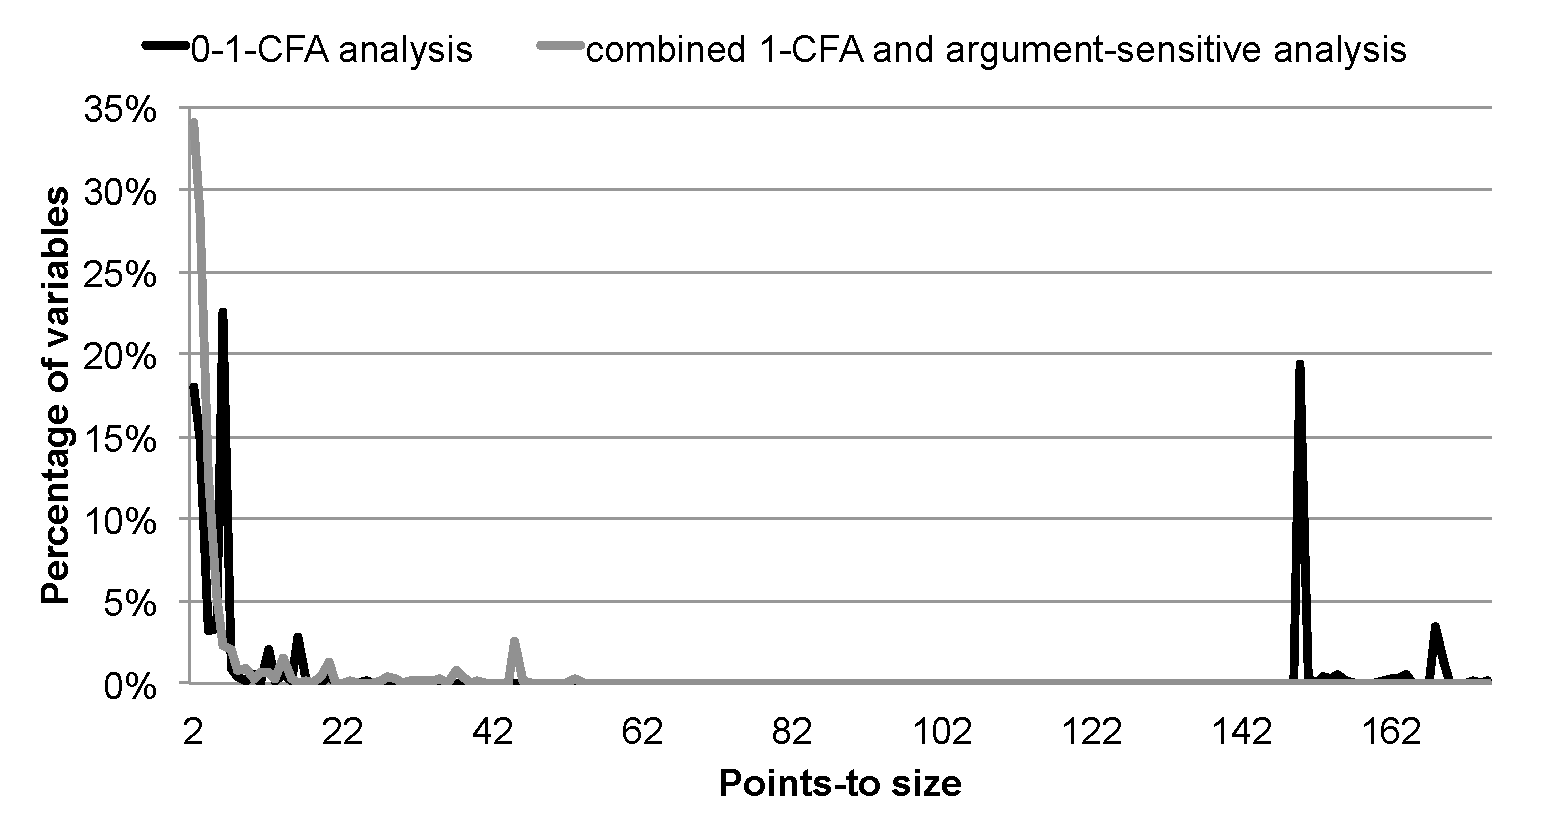
\includegraphics[width=\columnwidth]{pts-distribution}
\caption{\textmd{Points-to size distribution.}}
\label{fig:pts-distribution}
\end{figure}

Figure \ref{fig:pts-distribution} shows the distributions of the points-to sizes for each variable in the program. The x axis presents the points-to size of a variable and the y axis presents the percentage of the variables in the program with the corresponding points-to size. For the combined context-sensitive analysis, the points-to size of the majority of the variables (i.e., 81\%) is less than 6 and few variables are associated with large points-to sets. Interestingly for the 0-1-CFA analysis, the points-to sizes of only 40\% variables are less than 6 and there are condensed occurrences of variables with extremely large points-to sets (e.g., about 20\% of the variables' points-to sizes are 150). This result also indicates that overly-approximated results of specific program constructs may pollute many places in the program due to copying during the points-to propagations.

The above results demonstrate the significant different behaviors between points-to analyses when their performance and precision varies. These results motivated us to design an automated approach to identify root causes of imprecision via the differences of static analysis behavior. 

\subsection{Root Cause Localization \& Improvement Suggestion}

We now use the example in Figure \ref{fig:jquery-modified} to illustrate the ideas on localizing root causes. First, the root cause localization should be performed during the period in which overall precision of the points-to analysis starts to decrease, reflected as the ``jumps'' in terms of the overall points-to size in Figure \ref{fig:pts-growth}. Second, we use the history information of points-to propagations and the incomplete points-to results to locate the program constructs that are root causes of imprecision. Intuitively, two conditions should be met: (i) the program construct has a wide reach within the propagation system (e.g., the values of the property access {\tt source[name]} are assigned to property {\tt name} of {\tt target} at line 5 and are transitively propagated to about 500 other program variables or reference properties), and (ii) the impact of its wide reach is significant (e.g., looking up the property {\tt name} of {\tt source} at line 5 produces the points-to size of 150). Therefore, the imprecision of this property access results in the overall imprecision of the 0-1-CFA analysis when analyzing {\it jQuery} applications, becoming a root cause.

In addition, to further assist in the process of improving the results of static analysis, we design an improvement suggestion algorithm that uses dynamic information to suggest appropriate context sensitivity to improve the analysis precision on the identified root causes. The dynamic information is used to simulate the benefits of different context-sensitive analyses, a generally applicable idea to quantify the potential precision of a specific context sensitivity.

%because there are existing static analysis techniques that are designed to perform well for specific program constructs,

%Because of the high cost of locating analysis bottlenecks in programs, in this work we present automated bottleneck localization via program analysis based on the observations in terms of the points-to analysis behavior. We aim to locate the specific program variables as performance bottlenecks. Intuitively, two conditions should be met: 

%\begin{enumerate}
%	\item {\sf ptr} is (transitively) assigned to a large number of other pointer keys.
%	\item The points-to set of {\sf ptr} is large.
%\end{enumerate}
%By the first condition, {\sf ptr} has wide reach within the fixpoint system. By the second condition, the impact of its wide reach is significant. As an example, for 0-1-CFA analysis, looking up the property {\tt name} of {\tt source} at line 5 in Figure \ref{fig:jquery-modified} results in a large point-to set (i.e., 150 in size) and its values are assigned to property {\tt name} of {\tt target} and transitively to at least 30 other program variables. Therefore, the imprecision of this property accesses results in the overall imprecision of the 0-1-CFA analysis when analyzing {\it jQuery} applications, becoming an analysis bottleneck. Applying more accurate technique (e.g., \cite{Sridharan:2012:CTP:2367163.2367191}) at this specific program point may resolve the overall performance and precision issues. In this work, we have designed an automatic analysis that extracts the variable precision impact information from points-to analysis and locates the program locations that are analysis bottlenecks.

%In addition, we have also designed a automatic improvement suggestion algorithm that uses dynamic information to suggest appropriate context sensitivity to improve the analysis precision on bottlenecks. The dynamic information is used to animate the benefits of different context-sensitive analyses, a generally applicable idea to quantify the potential of context sensitivity precision on a subset of the functions in the program.

\begin{comment}
1. static analysis has issues with performance and precision, especially with dynamic features, and becomes useless.
    1.1 many JS analysis experiences performance issues; 
    1.2 it is difficult to manually reason about the causes of the issues (bottlenecks); 
    1.3 illustrate the second claim with example?
    
2. interesting behavior of useless analysis. 
     2.1 present the characteristics/behavior of useless and useful analysis, and compare.
     
3. the results from 2 lead us to design an analysis that analyzes the behavior of the useless analysis, (i) locates the bottlenecks, and (ii) propose possible fixes (with the same example)
\end{comment}

\begin{comment}
In this section, we walk the reader through an overview of our approach with reference to the code in Figure \ref{fig:jquery-extracted}, taken from the jQuery framework, for illustration purposes. [[ Can we say more about the example? ]]

\subsection{The Problem and Its Symptoms}

Static program analysis is challenged, by its very definition, by dynamic constructs like reflection. This is among the greatest challenges in JavaScript analysis, where reflective capabilities --- such as enumeration over, and access to, an object's properties --- are baked into the core syntax. Examples of this, in Figure \ref{fig:jquery-extracted}, are the {\sf for} loop iterating over property identifiers at lines XXX, YYY and ZZZ. Other challenging constructs include closures, variadic function, prototype-chain lookup, etc.

These (and other) challenges have significant impact on the precision of Andersen-style analysis of real-world JavaScript programs. In the absence of special treatment for challenging constructs, the analysis becomes overly conservative, losing track of correlations that are critical for acceptable precision. For the code in Figure \ref{fig:jquery-extracted}, for instance, the analysis would propagate pointers across every pair of properties in {\sf source} and {\sf target}, which is detrimental to its precision.

Importantly, however, at the lower level of the fixpoint system computing the points-to solution, these challenges are all abstracted into the same symptom: excessively large points-to sets due to infeasible pointer flows. As an illustration, 
we refer the reader to Figure \ref{fig:pts-growth}, which depicts the evolution of the points-to graph (measured as the number of points-to edges) for a simple client of jQuery v1.6.1 as a function of fixpoint iterations.

In the figure, there are two trend lines. The red ``linear'' line corresponds to 1-CFA analysis with argument sensitivity, and the other line to 0/1-CFA. As 0/1-CFA is more coarse, important dimensions of precision are lost, and the analysis fails to complete within a time budget of 10 minutes. Comparatively, the 1-CFA analysis finishes in under 5 seconds.

These behaviors are reflected in the trend lines. While the 1-CFA points-to graph grows at a steady rate, the 0-CFA line exhibits a jerky behavior with step-like jumps. These correspond to the symptoms mentioned above: large points-to sets reaching wide regions in the points-to graph.

\subsection{Step I: Diagnosis}

Our first observation, enabling diagnostic analysis, concerns the detemrmination whether a given pointer variable (or pointer key) {\sf ptr} is conducive to accuracy loss. For {\sf ptr} to qualify as such, two conditions should be met:
\begin{enumerate}
	\item {\sf ptr} is (transitively) assigned to a large number of other pointer keys.
	\item The points-to set of {\sf ptr} is large.
\end{enumerate}
By the first condition, {\sf ptr} has wide reach within the fixpoint system. By the second condition, the impact of its wide reach is significant.

As an example, ... [[ point to motivating example and show a fragment of points-to graph ]].

To enforce the diagnostic conditions above, we instrument the fixpoint system to track flow of pointer keys. Given a dataflow equation $e$ propagating points-to elements between pointer keys {\sf x} and {\sf y}, where {\sf y} has points-to set $S$, we instrument the points-to edge ${\sf y} \mapsto S$ to include {\sf x}: ${\sf y} \stackrel{{\sf x}}{\mapsto} S$.

Tracking pointer keys as edge labels addresses the first condition above. Evaluating the second condition is straightforward. Deriving the size of the points-to set of a given pointer key is immediate from the points-to graph.

\subsection{Step II: Remediation}

Having identified precision bottlenecks, in the form of pointer variables requiring additional sensitivity, we turn to the remediation problem. We propose a heuristic, based on (i) a parametric library of sensitivity policies as well as (ii) a dynamic analysis to simulate their effects w.r.t. concrete runtime states and compare between them, to recommend to the analysis designer how to refine the analysis.

\paragraph{Sensitivity Policies.} The problem of imprecision in JavaScript points-to graphs has been observed, and addressed, in various studies. Beyond that, there are general schemes to add sensitivity to a propagation-based call graph. In this paper, we focus on the following sensitivity policies in particular:
\begin{itemize}
	\item XXX
	\item YYY
	\item ZZZ
	\item ...
\end{itemize}

\paragraph{Recommendation Algorithm.} Given the library $\{ s_1,\ldots, s_n \}$ of sensitivity policies, the recommendation which (type of) sensitivity to add is based on simulating the effects of the different policies $s_i$ w.r.t. a fully concrete points-to graph computed dynamically. Policy $s$ is considered better than $s'$ if XXX.

The motivation for using dynamic analysis is to be able to quantify the precision loss, or ambiguity, introduced by a given policy. That is, we can reason fully precisely about the concrete points-to facts that are smushed together due to a given policy.

To compute the points-to graph dynamically, we instrument the JavaScript program. This is done via XXX. The instrumented program is, on average, xYYY slower compared to the original version. We handle XXX...

For the example in Figure \ref{fig:jquery-extracted}, our solution correctly picks ...




proceeds by instrumenting the subject program to record, at runtime, the concrete --- and thus fully precise --- points-to graph $G^c$. The question of which sensitivity to recommend to the analysis designer then 



\subsection{Motivating Example}
In this section, we would like to use a code example (or a series of examples; see below) to demonstrate the difficulties to (manually) find the performance bottleneck of a static analysis. For example, Figure \ref{fig:jquery-orig} shows the original {\tt extend} function of jQuery whose behavior is not easy to understand; moreover, due to its usage of complicated program structures (e.g., recursion, function variadicity), it is difficult for an analysis to accurately model the results of this function (confirmed in \cite{}). In \cite{}, the authors had to manually transform this function to simplify its structure, resulting in the code in Figure \ref{fig:jquery-modified}. Nevertheless, the transformed code, in and of itself, is still insufficient for a field-sensitive analysis to complete analyzing simple jQuery applications. Therefore, the authors of \cite{} designed an automatic function extraction algorithm (correlation extraction) and used argument sensitivity to improve the performance and precision of JavaScript points-to analysis. The code that is actually being analyzed by the argument-sensitive analysis is presented in Figure \ref{fig:jquery-extracted}. Overall, the take-away message shall be: it is difficult to locate the analysis bottleneck and it is also difficult to find a solution to improve the analysis. This series of examples strongly support the above statement: (1) among almost 9,000 lines of code of jQuery library, it usually is clueless to know that one particular function results in the analysis performance bottleneck (without investigating the code); (2) even if the analysis designer is able to locate this function as the bottleneck, it is difficult to tell which program structure or if it is the combination of several program structures that result in bad analysis behavior, thus making it difficult to develop new technology to improve the analysis; (3) even if the analysis designer is able to (manually) abstract away several challenges (e.g., the transformed function in Figure \ref{fig:jquery-modified}), and wants to apply the more precise technique whole program (e.g., argument sensitivity), this may in turn results in overhead because the other portion of the program may not benefit from the more advanced technique (although this particular function will significantly benefit from argument sensitivity). ({\bf Comment from Shiyi: despite that I think this is a good series examples as motivation, we cannot afford to use too much space for the codes; simplify the code, especially Figure 1 (included the complete code for your reference), as the ECOOP 12 paper did; or use one whole example to demonstrate what we want to express. Also, note that our technique does not automatically fixes the issues discussed in (1) and (2) above, while we do locate the bottleneck function and apply the advanced techniques, thus solving problem (3) above.}).

\begin{figure}[th!]
        \lstinputlisting{jquery-orig.js}
\caption{\textmd{Original {\tt extend} function of jQuery 1.6.1.}}
\label{fig:jquery-orig}
\end{figure}

\begin{figure}[th!]
        \lstinputlisting{jquery-extracted.js}
\caption{\textmd{Mofified {\tt extend} function with correlation extraction \cite{} of jQuery 1.6.1}}
\label{fig:jquery-extracted}
\end{figure}

\subsection{Static Points-to Analysis Behavior (Empirical Study)}
To (manually or automatically) understand and debug the performance and precision issues associated with static points-to analysis, it is important to know its behavior (normal and abnormal). We present some data to characterize the points-to analysis behavior.

1. growth of points-to graph size (points-to edges) during points-to analysis lifetime. Figure \ref{fig:pts-growth} shows the growth rate of two points-to analyses on an application that invokes jQuery 1.6.1 library. The bad points-to analysis is the baseline analysis (i.e., 0-1-cfa) which could not finish under limited time budget (10 minutes); the good points-to analysis is a 1-cfa and argument-sensitive which finishes analyzing the program in less than 5 seconds and the total number of points-to iteration is about 118,000. Comparing the life time of the bad (part of its lifetime as its lifetime could be much longer) and the good points-to analysis, we observe the growth rate of points-to size (i.e., we count the total number of points-to edges in the graph every 5000 iterations) of good points-to analysis is steady while the bad points-to analysis has ``jumps" (indicating the approximation and "pollution" of points-to results). This finding motivated us to design heuristics to decide when we would like to perform the automatic diagnostic analysis for a bad analysis (i.e., when the slope of growth significantly change). ({\bf Comment by Shiyi: the data of Figure \ref{fig:pts-growth} is included in section2-results.xlsx. I think this is interesting and we may need one more figure on other programs to better support our argument.})



2. Points-to size (per pointer key) distribution. See section2-results.xlsx for the data (columns I and J). The data show very interesting and different characteristics of points-to size distribution between a good and bad points-to analyses (the same analyses as in Figure \ref{fig:pts-growth}). We collected this data for each analysis after 100,000 iterations. I think we are looking for a frequency graph here that x axis represents the size of points-to size and y axis represents the number of pointer keys with the specific size of points-to set. Roughly looking at the data, for example in column I (the good points-to analysis), the curve is likely to evenly going down with the increase of points-to size. While for the bad points-to analysis (column J), the curve seems evenly going down with the increase of points-to size until the size of 33; after 33, the next size jumps to 150, and there are a lot of pointer keys with points-to size greater than 150 (thus, the frequency graph/curve/histogram would grow after specific number for the bad analysis). This result is interesting in that this indicates for a bad points-to analysis, some approximate results polluted a lot of places in the graph; thus making the analysis unscalable and extremely imprecise. ({\bf Comment by Shiyi: I can use excel to generate the frequency graph, but it may take some time for me to do so, but I do think this result is interesting to report because the "outliers" (i.e., many pointer keys with large points-to size) in the bad points-to graph indicate how the bottleneck can pollute the analysis and that motivates us find the bottleneck. Furthermore, taking close look at the "large" points-to sizes, many pointer keys share the same points-to sizes, indicating that many could be copies from previously approximate results; thus being "polluted" after copying. This finding motivates us to track the copies of points-to sets during the diagnosis.})

3... We may think of more to report on points-to analysis characteristics. We shall focus on the characteristics that distinguish the good and bad points-to analysis. More data make this subsection an empirical study of static points-to analysis behavior and characterization of good/bad points-to analysis, which in and of itself is a good effort and something new to present, thus making it a contribution of this paper.

({\bf Further comments on Section 2 by Shiyi: I think with the empirical study, this section can be long, but it is Ok as we already are presenting new observations and findings in this section. These new findings very well serve the motivation and design guidance of our algorithm; thus very tightly connected to the rest of the paper.})
\end{comment}